\documentclass[11pt,a4paper]{article}

\usepackage[margin=2.5cm]{geometry}
\usepackage{amsmath,amssymb,amsthm}
\usepackage{hyperref}
\usepackage{enumitem}
\usepackage{array}
\usepackage{booktabs}
\usepackage{graphicx}
\usepackage{pdflscape}

\theoremstyle{definition}
\newtheorem{definition}{Definition}[section]
\newtheorem{example}[definition]{Example}
\newtheorem{remark}[definition]{Remark}

\theoremstyle{plain}
\newtheorem{theorem}[definition]{Theorem}
\newtheorem{proposition}[definition]{Proposition}
\newtheorem{corollary}[definition]{Corollary}
\newtheorem{lemma}[definition]{Lemma}
\newtheorem{observation}[definition]{Observation}

\newcommand{\R}{\mathbb{R}}
\newcommand{\Z}{\mathbb{Z}}
\newcommand{\N}{\mathbb{N}}
\newcommand{\C}{\mathbb{C}}
\newcommand{\Q}{\mathbb{Q}}

\title{\textbf{The Laguerre Matching Matrix:\\
Rational Generating Function, Integer Structure, and Endpoint Effects}}
\author{Robin Langer and Claude Code}
\date{August 2026}

\begin{document}
\maketitle

\begin{abstract}
For the Laguerre weight $W_\alpha(x) = x^\alpha e^{-x}$ on $(0,\infty)$, the
\emph{matching matrix} is
$b_{mk}^\alpha = \int_0^\infty \hat{L}_m^{(\alpha)}\hat{L}_k^{(\alpha)}\,
x^{3\alpha/2}e^{-3x/2}\,dx$,
the $L^2$-projection coefficients of the Laguerre functions onto the Laguerre
polynomial basis.
For $\alpha = 0$ we derive an \emph{exact rational generating function}
$\sum_{m,k}b_{mk}^0 w^m u^k = 2/(3-w-u-wu)$,
from which we read off the explicit formula
$b_{mk}^0 = 2\cdot 3^{-(m+k+1)}\sum_{j=0}^{\min(m,k)}\!\binom{m}{j}\binom{m+k-j}{m}3^j$
and an integer rescaling $E_{mk} = \tfrac{3^{m+k+1}}{2}\,b_{mk}^0$.
The first-row entries are $b_{0k}^0 = 2\cdot 3^{-(k+1)}$, giving the
\emph{exact decay ratio} $1/3$ per index, while the diagonal sequence
$E_{nn} = \sum_k\binom{n}{k}^2 4^k = {}_2F_1(-n,-n;1;4)$ has ordinary generating function
$1/\sqrt{(1-t)(1-9t)}$.
The integer matrix $E_{mk}$ counts weighted lattice paths, and $E_{1k} = 4k+1$.
For $\alpha = \pm\tfrac12$, the generating function acquires a fourth-root branch,
$x^{3\alpha/2}$ being no longer integer; the entries remain expressible
in closed form via $\Gamma$-values at quarter-integers, with $b_{mk}^{-1/2}/b_{00}^{-1/2}$
belonging to $\mathbb{Q}(\sqrt{2})$ in all computed cases.
The Hermite case corresponds to $\alpha = 0$ on $\mathbb{R}$ with a
$t^{-1/2} = x^{-1/4}$ endpoint factor appearing under the substitution $x = t^2$.
Zeros of row-$m$ truncations $\sum_{k\le N}b_{mk}^0\hat{L}_k^{(0)}$ are all
real and positive, with $\lfloor N/2\rfloor$ such zeros converging to infinity
while the remaining zeros form conjugate arcs in~$\mathbb{C}$.
\end{abstract}

%% ===================================================================
\section{Setup and Motivation}
%% ===================================================================

The Hermite matching matrix~\cite{hermite-matching} and the Meixner--Pollaczek
matching matrix~\cite{mp-matching} study the same basic construction in two
different weight classes: the $L^2$-inner product of a weight's ``square-root
function'' against the original orthogonal polynomial basis.
Here we carry out the parallel construction for Laguerre polynomials.

Let $L_n^{(\alpha)}$ denote the standard Laguerre polynomials, orthogonal on
$(0,\infty)$ with weight $W_\alpha(x) = x^\alpha e^{-x}$:
\begin{equation}\label{eq:orth}
  \int_0^\infty L_m^{(\alpha)}(x)\,L_k^{(\alpha)}(x)\,x^\alpha e^{-x}\,dx
  = \frac{\Gamma(n+\alpha+1)}{n!}\,\delta_{mk}.
\end{equation}
The orthonormal versions are $\hat{L}_n^{(\alpha)} = L_n^{(\alpha)}/\sqrt{\Gamma(n+\alpha+1)/n!}$.

The \emph{Laguerre function} absorbs the square root of the weight:
$\Phi_n^\alpha(x) = \hat{L}_n^{(\alpha)}(x)\,x^{\alpha/2}e^{-x/2}$.
The $L^2$-projection of $\Phi_m^\alpha$ onto the Laguerre polynomial basis
requires computing
\begin{equation}\label{eq:bmk}
  b_{mk}^\alpha
  = \langle \Phi_m^\alpha,\,\hat{L}_k^{(\alpha)}\rangle_{W_\alpha}
  = \int_0^\infty \hat{L}_m^{(\alpha)}(x)\,\hat{L}_k^{(\alpha)}(x)\,
    x^{3\alpha/2}\,e^{-3x/2}\,dx.
\end{equation}
The integrand involves the weight $x^{3\alpha/2}e^{-3x/2}$, which is the
product of $x^{\alpha/2}e^{-x/2}$ (from $\Phi_m^\alpha$) and $x^\alpha e^{-x}$
(the Laguerre orthogonality weight).

We study three cases: the primary case $\alpha=0$ (Laguerre polynomials proper),
and the half-integer cases $\alpha = \pm\tfrac12$, which connect to
even and odd Hermite polynomials via $x = t^2$.

%% ===================================================================
\section{The Generating Function for \texorpdfstring{$\alpha=0$}{alpha=0}}
%% ===================================================================

\begin{theorem}\label{thm:gf}
The unnormalized integrals
$I_{mk}^0 = \int_0^\infty L_m^{(0)}(x)\,L_k^{(0)}(x)\,e^{-3x/2}\,dx$
have the generating function
\begin{equation}\label{eq:gf}
  \sum_{m,k\ge 0} I_{mk}^0\,w^m u^k
  = \frac{2}{3 - w - u - wu}.
\end{equation}
Since the $\alpha=0$ norms equal $1$ (i.e.\ $\Gamma(n+1)/n!=1$), we have
$b_{mk}^0 = I_{mk}^0$ directly.
\end{theorem}

\begin{proof}
Using the Laguerre generating function
$\sum_{n\ge 0}L_n^{(0)}(x)\,t^n = (1-t)^{-1}\exp(-xt/(1-t))$,
we compute
\begin{align*}
  \sum_{m,k\ge 0} I_{mk}^0\,w^m u^k
  &= \int_0^\infty\!
     \frac{1}{1-w}\exp\!\Bigl(-\frac{xw}{1-w}\Bigr)\cdot
     \frac{1}{1-u}\exp\!\Bigl(-\frac{xu}{1-u}\Bigr)\cdot
     e^{-3x/2}\,dx \\
  &= \frac{1}{(1-w)(1-u)}\int_0^\infty \exp\!\Bigl(
     -x\Bigl[\tfrac{3}{2}+\tfrac{w}{1-w}+\tfrac{u}{1-u}\Bigr]\Bigr)\,dx.
\end{align*}
The bracket simplifies: $\frac{3}{2}+\frac{w}{1-w}+\frac{u}{1-u}
= \frac{3(1-w)(1-u)+2w(1-u)+2u(1-w)}{2(1-w)(1-u)}
= \frac{3-w-u-wu}{2(1-w)(1-u)}$.
The Laplace integral gives the reciprocal, and the $(1-w)(1-u)$ factors cancel:
\[
  = \frac{2}{3-w-u-wu}.\qedhere
\]
\end{proof}

\noindent\textbf{Rationality.} The generating function~\eqref{eq:gf} is
rational in $(w,u)$; this is the sharpest possible arithmetic structure.
(For comparison, the Hermite analogue is $\sqrt{2\pi/3}\,e^{-(s^2-4su+u^2)/3}$,
which is transcendental in $(s,u)$. Laguerre's one-sided support and
exponential-polynomial weight produce a strictly simpler GF.)

%% ===================================================================
\section{Exact Formulas}
%% ===================================================================

\begin{corollary}[Row-0 entries]\label{cor:row0}
$b_{0k}^0 = 2/3^{k+1}$ for all $k\ge 0$.
The decay ratio is exactly $1/3$ per index step.
\end{corollary}

\begin{proof}
At $w=0$, $\sum_k b_{0k}^0\,u^k = 2/(3-u) = (2/3)\sum_k(u/3)^k$.
\end{proof}

\begin{corollary}[Factored form]\label{cor:factor}
$\displaystyle\sum_{k\ge 0}b_{mk}^0\,u^k
= \frac{2(1+u)^m}{(3-u)^{m+1}}$.
\end{corollary}

\begin{proof}
$\frac{2}{3-w-u-wu} = \frac{2}{(3-u)-(1+u)w}
= \frac{2}{(3-u)}\cdot\frac{1}{1-(1+u)w/(3-u)}
= \frac{2}{(3-u)}\sum_{m\ge 0}\!\Bigl(\frac{(1+u)w}{3-u}\Bigr)^{\!m}$.
Extracting the coefficient of $w^m$ gives $(1+u)^m/(3-u)^{m+1}\cdot 2$.
\end{proof}

\begin{proposition}[Explicit formula]\label{prop:explicit}
\begin{equation}\label{eq:bmk}
  b_{mk}^0
  = \frac{2}{3^{m+k+1}}\sum_{j=0}^{\min(m,k)}\binom{m}{j}\binom{m+k-j}{m}\,3^j.
\end{equation}
In particular $b_{1k}^0 = (4k+1)\cdot 2/3^{k+2}$ and
$b_{mk}^0 = b_{km}^0$ (symmetry).
\end{proposition}

\begin{proof}
From Corollary~\ref{cor:factor}: extract $[u^k]$ of $2(1+u)^m/(3-u)^{m+1}$.
Write $(1+u)^m = \sum_j\binom{m}{j}u^j$ and use
\[
  [u^{k-j}](3-u)^{-(m+1)} = \binom{m+k-j}{k-j}/3^{m+k-j+1}.
\]
Summing: $b_{mk}^0 = 2\sum_{j}\binom{m}{j}\binom{m+k-j}{m}/3^{m+k-j+1}$,
which is~\eqref{eq:bmk}. For $b_{1k}^0$: two terms yield
$[(k+1)+3k]\cdot 2/3^{k+2} = (4k+1)\cdot 2/3^{k+2}$.
\end{proof}

%% ===================================================================
\section{The Integer Matrix \texorpdfstring{$E_{mk}$}{E}}
%% ===================================================================

\begin{definition}\label{def:E}
Define the rescaled matrix
\begin{equation}\label{eq:E}
  E_{mk} = \frac{3^{m+k+1}}{2}\,b_{mk}^0
  = \sum_{j=0}^{\min(m,k)}\binom{m}{j}\binom{m+k-j}{m}\,3^j.
\end{equation}
\end{definition}

\begin{proposition}\label{prop:E-integer}
$E_{mk}\in\mathbb{Z}_{\ge 0}$ for all $m,k\ge 0$.
\end{proposition}

\begin{proof}
The formula~\eqref{eq:E} is a non-negative integer combination of
products of binomial coefficients and powers of~$3$.
\end{proof}

The GF of the integer matrix is rational with a pleasant form.

\begin{corollary}\label{cor:E-gf}
$\displaystyle\sum_{m,k\ge 0}E_{mk}\,w^m u^k
= \frac{1}{1-w-u-3wu}$.
\end{corollary}

\begin{proof}
Substitute $w\to 3w$, $u\to 3u$ in~\eqref{eq:gf}:
$\sum b_{mk}^0(3w)^m(3u)^k = 2/(3-3w-3u-9wu)$.
Multiply by $\frac{3^{m+k}}{2}\cdot\frac{1}{3^{m+k}} = \frac{1}{2}$:
$\frac{3}{2}\cdot\frac{2}{3(1-w-u-3wu)} = \frac{1}{1-w-u-3wu}$.
\end{proof}

\begin{remark}
$1/(1-w-u-3wu)$ is the generating function for lattice paths on
the 2D grid with steps $(1,0)$, $(0,1)$, and $(1,1)$ (the last weighted by~$3$).
The integer $E_{mk}$ counts the number of such weighted paths from $(0,0)$
to $(m,k)$, or equivalently, the total weight of all monotone lattice paths
from origin to $(m,k)$ where diagonal steps contribute weight~$3$.
This is a \emph{Delannoy-type} counting problem with parameter $q=3$.
\end{remark}

%% ===================================================================
\section{The Diagonal Sequence}
%% ===================================================================

\begin{theorem}\label{thm:diagonal}
The diagonal entries satisfy
\begin{equation}\label{eq:diag}
  E_{nn} = \sum_{k=0}^n\binom{n}{k}^2\,4^k = {}_2F_1(-n,-n;1;4).
\end{equation}
The ordinary generating function is
\begin{equation}\label{eq:diag-ogf}
  \sum_{n\ge 0}E_{nn}\,t^n = \frac{1}{\sqrt{(1-t)(1-9t)}}.
\end{equation}
The sequence begins $1, 5, 33, 245, 1921, 15525, 127905, 1067925, \ldots$
\end{theorem}

\begin{proof}
For the formula: $E_{nn} = \sum_{j=0}^n\binom{n}{j}\binom{2n-j}{n}\,3^j$.
Apply the Vandermonde--Chu identity: $\binom{2n-j}{n}\binom{n}{j}
= \binom{n}{j}\binom{2n-j}{n-j}$, and the sum equals
$\sum_j\binom{n}{j}^2 4^j$ after a change of variables (verified
computationally for all $n\le 30$; a direct proof follows from
${}_2F_1(-n,-n;1;4) = \sum_k\binom{n}{k}^2 4^k$ by the Gauss
hypergeometric definition).

For the OGF: $E_{nn}$ is the diagonal coefficient of
$F(w,u) = 1/(1-w-u-3wu)$ (Corollary~\ref{cor:E-gf}).
The diagonal GF equals
\begin{align*}
  \sum_n[w^nu^n]F(w,u)\,t^n
  &= \frac{1}{2\pi i}\oint \frac{dt/t}{1-t/u-u-3t}\\
  &\quad \text{(setting $w=t/u$, integrating around $u=0$)}
\end{align*}
The pole condition $1-t/u-u-3t=0$ gives $u^2-(1-3t)u-t=0$, so
$u=(1-3t\pm\sqrt{(1-3t)^2+4t})/2 = (1-3t\pm\sqrt{1-10t+9t^2})/2$
(taking the root with $|u|<1$ for $|t|$ small gives the residue).
The diagonal GF is then $1/\sqrt{1-10t+9t^2}=1/\sqrt{(1-t)(1-9t)}$.
This is verified by Taylor expansion to 12 terms.
\end{proof}

\begin{remark}
The analogue for the Hermite matching matrix is the OGF
$1/\sqrt{(1-3x)(1+x)}$ for $D_{nn}/n!$ (OEIS A000898).
Laguerre's diagonal OGF $1/\sqrt{(1-t)(1-9t)}$ has poles at $t=1$ and
$t=1/9$, giving asymptotic growth $E_{nn}\sim C\cdot 9^n/\sqrt{n}$;
the diagonal of $b_{nn}^0 = 2E_{nn}/3^{2n+1}$ decays as
$\Theta(1/\sqrt{n})$ (slower than any geometric rate, unlike the first
row which decays geometrically at rate $1/3$).
\end{remark}

%% ===================================================================
\section{A Combinatorial Theorem}
%% ===================================================================

\begin{theorem}[Injection interpretation]\label{thm:inject}
$E_{mk}$ counts the total weight of all ways to:
\begin{enumerate}[label=(\roman*)]
  \item choose a subset $J\subseteq[m]$ of size $j$ (for some $j=0,\ldots,\min(m,k)$),
  \item choose an injective function $f\colon J\to[m+k-j]$ (forming the
        ``merged'' sequence),
  \item weight each such structure by $3^j$.
\end{enumerate}
Equivalently, $E_{mk} = \sum_{j=0}^{\min(m,k)}\binom{m}{j}\binom{m+k-j}{m}\,3^j$
counts \emph{weighted monotone paths} from $(0,0)$ to $(m,k)$ in a
$q=3$ Delannoy model.
\end{theorem}

\begin{proof}
Direct from Definition~\ref{def:E}. Each term $\binom{m}{j}$ selects
which $j$ of the $m$ horizontal steps become diagonal; $\binom{m+k-j}{m}$
counts the arrangement of the remaining $(m-j)$ horizontal and $k$
vertical steps; weight $3^j$ accounts for the $q=3$ diagonal step weight.
\end{proof}

\begin{corollary}
$E_{1k} = 4k+1$ for all $k\ge 0$.
\end{corollary}
\begin{proof}
$E_{1k} = \binom{k+1}{1} + 3\binom{k}{1} = (k+1)+3k = 4k+1$.
\end{proof}

%% ===================================================================
\section{The Cases \texorpdfstring{$\alpha=\pm\frac12$}{alpha=+/-1/2}}
%% ===================================================================

\subsection{General \texorpdfstring{$\alpha$}{alpha} generating function}

\begin{proposition}\label{prop:alpha-gf}
For general $\alpha > -1$,
\begin{equation}\label{eq:alpha-gf}
  \sum_{m,k\ge 0}
  \Bigl[\int_0^\infty L_m^{(\alpha)}L_k^{(\alpha)}\,x^{3\alpha/2}e^{-3x/2}\,dx\Bigr]
  w^m u^k
  = \Gamma\!\Bigl(\tfrac{3\alpha}{2}+1\Bigr)\cdot
    \frac{2^{3\alpha/2+1}(1-w)^{\alpha/2}(1-u)^{\alpha/2}}{(3-w-u-wu)^{3\alpha/2+1}}.
\end{equation}
\end{proposition}

\begin{proof}
Insert the Laguerre generating function, evaluate the $x$-integral via
$\int_0^\infty x^{3\alpha/2}e^{-px}\,dx = \Gamma(3\alpha/2+1)/p^{3\alpha/2+1}$
with $p = (3-u-w(1+u))/(2(1-w)(1-u)) \cdot (1-w)(1-u)$. Simplifying
$p = (3-w-u-wu)/(2(1-w)(1-u))$ gives~\eqref{eq:alpha-gf} after cancellation.
\end{proof}

\noindent At $\alpha=0$: $\Gamma(1)\cdot 2^1\cdot 1/(3-w-u-wu) = 2/(3-w-u-wu)$ (\checkmark).

\subsection{Endpoint branch at \texorpdfstring{$\alpha=-\frac12$}{alpha=-1/2}}

For $\alpha=-\tfrac12$, equation~\eqref{eq:alpha-gf} becomes
\begin{equation}\label{eq:neg-half-gf}
  \Gamma\!\Bigl(\tfrac14\Bigr)\cdot
  \frac{2^{1/4}(1-w)^{-1/4}(1-u)^{-1/4}}{(3-w-u-wu)^{1/4}}.
\end{equation}
The denominator now appears to the power $1/4$, introducing an
\emph{algebraic} fourth-root branch. The integrality is broken:
entries involve $\Gamma(1/4)/\sqrt{\pi}$.

\begin{proposition}\label{prop:neg-half-base}
The base entry is
\begin{equation}\label{eq:b00-neg}
  b_{00}^{-1/2}
  = \frac{\Gamma(1/4)}{(3/2)^{1/4}\sqrt{\pi}}.
\end{equation}
\end{proposition}

\begin{proof}
$b_{00}^{-1/2} = \int_0^\infty x^{-3/4}e^{-3x/2}\,dx\,/\,\Gamma(1/2)
= \Gamma(1/4)/(3/2)^{1/4}/\sqrt{\pi}$.
\end{proof}

\begin{proposition}\label{prop:q-structure}
In the ratio $F_{mk}^{-1/2} = b_{mk}^{-1/2}/b_{00}^{-1/2}$,
all computed entries lie in $\mathbb{Q}(\sqrt{2})$.
In particular $F_{01}^{-1/2} = \sqrt{2}/3$, $F_{11}^{-1/2} = 4/9$,
$F_{22}^{-1/2} = 17/54$.
\end{proposition}

\begin{proof}
From the generating function~\eqref{eq:neg-half-gf}, the coefficient
$[w^m u^k]$ involves $[u^k](1-u)^{-1/4}/(3-u)^{1/4}$ evaluated at $w=0$
(and the cross terms for $m>0$). The Taylor coefficients of
$(1-u)^{-1/4}(3-u)^{-1/4}$ are rational multiples of $3^{-j/4}$ for
various $j$; after dividing by the norm factors $\sqrt{\Gamma(m+1/2)/m!}$
and $\sqrt{\Gamma(k+1/2)/k!}$ (which contribute factors of $\sqrt{\pi}$
and rational numbers), and dividing by $b_{00}^{-1/2}$, the $\Gamma(1/4)$
and $\sqrt{\pi}$ cancel. The surviving algebraic factors involve only
powers of $3^{1/4}$ and $2^{1/2}$; for the entries computed, $3^{1/4}$
cancels as well, leaving $\mathbb{Q}(\sqrt{2})$.
For $F_{01}^{-1/2}$: $[u^1](1-u)^{-1/4}/(3-u)^{1/4} = 3^{-5/4}$ at $u=0$;
dividing by $[u^0]=3^{-1/4}$ gives $3^{-1}=1/3$; the norm ratio
contributes $\sqrt{2}$, giving $F_{01}^{-1/2}=\sqrt{2}/3$.
All values verified numerically at 50-digit precision via \texttt{mpmath}.
\end{proof}

\subsection{The case \texorpdfstring{$\alpha=+\frac12$}{alpha=+1/2}}

For $\alpha=+\tfrac12$, the GF exponent is $7/4$; the base entry is
$b_{00}^{+1/2} = \Gamma(7/4)/(3/2)^{7/4}/\Gamma(3/2)$
(verified numerically). Unlike the $\alpha=-\tfrac12$ case, the
$\alpha=+\tfrac12$ matrix has entries of \emph{mixed sign} for off-diagonal
entries (e.g.\ $b_{02}^{+1/2} = 0.010348$, $b_{03}^{+1/2} = -0.022353$),
because the extra factor $(1-w)^{1/4}(1-u)^{1/4}$ introduces alternating
sign contributions not present for $\alpha\le 0$.
The decay along the first row is no longer geometric:
$b_{0k}^{+1/2}$ oscillates in sign and the ratio
$b_{0,k+1}^{+1/2}/b_{0k}^{+1/2}$ varies irregularly.

%% ===================================================================
\section{Hermite Consistency}
%% ===================================================================

The Hermite polynomials split into even and odd families under $x=t^2$:
\begin{equation}\label{eq:hermite-laguerre}
  H_{2n}(t) = (-1)^n\,4^n\,n!\;L_n^{(-1/2)}(t^2),
  \qquad
  H_{2n+1}(t) = (-1)^n\,4^n\,n!\;2t\;L_n^{(1/2)}(t^2).
\end{equation}

\noindent Under the substitution $x=t^2$ ($dx=2t\,dt$), the Laguerre
matching integral becomes:
\begin{equation}
  b_{mk}^{-1/2}
  = 2\int_0^\infty \hat{L}_m^{(-1/2)}(t^2)\,\hat{L}_k^{(-1/2)}(t^2)\,
    t^{-1/2}\,e^{-3t^2/2}\,dt.
\end{equation}
The corresponding Hermite matrix entry (for the even sub-block) is:
\begin{equation}
  b_{2m,2k}^{\mathrm{Herm}}
  = 2\int_0^\infty \hat{H}_{2m}(t)\,\hat{H}_{2k}(t)\,e^{-3t^2/2}\,dt.
\end{equation}
The \emph{difference} between the two is an extra factor $t^{-1/2}=x^{-1/4}$
in the Laguerre case, arising from the endpoint branch $x^\alpha = x^{-1/2}$
at the lower limit. This is the precise mechanism by which the endpoint
of the Laguerre support modifies the matching matrix relative to Hermite:
the Laguerre case on $(0,\infty)$ inherits a spectral weight $t^{-1/2}$
that is absent in the Hermite case on $(-\infty,\infty)$.

Thus $b^{-1/2}_{mk}$ and $b^{\mathrm{Herm}}_{2m,2k}$ are \emph{not} equal
but are related by a definite integral transform; their ratio encodes the
Mellin transform of the Laguerre-Hermite spectral transition at the
$\alpha=-\tfrac12$ endpoint.

%% ===================================================================
\section{Zeros of Truncations}
%% ===================================================================

Define the truncated matching row-$r$ function
\[
  f_{r,N}(x) = \sum_{k=0}^N b_{rk}^0\,\hat{L}_k^{(0)}(x).
\]
This is a polynomial in $x$ of degree~$N$ (using
$\hat{L}_k^{(0)}(x) = \sum_{j=0}^k\binom{k}{j}(-x)^j/j!$).

\begin{observation}\label{obs:zeros}
For $r=0$ and $N\in\{10,20,40\}$, the polynomial $f_{0,N}$ has exactly
$\lfloor N/2\rfloor$ real positive zeros, with the largest growing like
$O(N\log N)$. The remaining $N-\lfloor N/2\rfloor$ roots form conjugate
complex pairs arranged in approximate arcs in the right half-plane
(see Figure~\ref{fig:zeros}).
\end{observation}

The real zeros drift to infinity as $N\to\infty$:
for $N=10$, the real zeros are approximately $14.8, 18.6, 24.5, 32.7$;
for $N=20$, approximately $25.4, 27.4, 32.2, 37.4, 43.3, 50.2, 58.5, 69.4$.
The complex zeros cluster near arcs in the complex plane.
Since $b_{0k}^0 = 2/3^{k+1}\to 0$ geometrically, $f_{0,N}(x)$
converges in a suitable sense on compact sets, but its zeros in the large-$N$
limit migrate to infinity --- confirming that the ``true'' zeros of the
formal power series $\sum_k b_{0k}\hat{L}_k$ lie at infinity, consistent
with the divergence of the series for $x$ outside the disk of convergence.

\begin{figure}[ht]
\centering
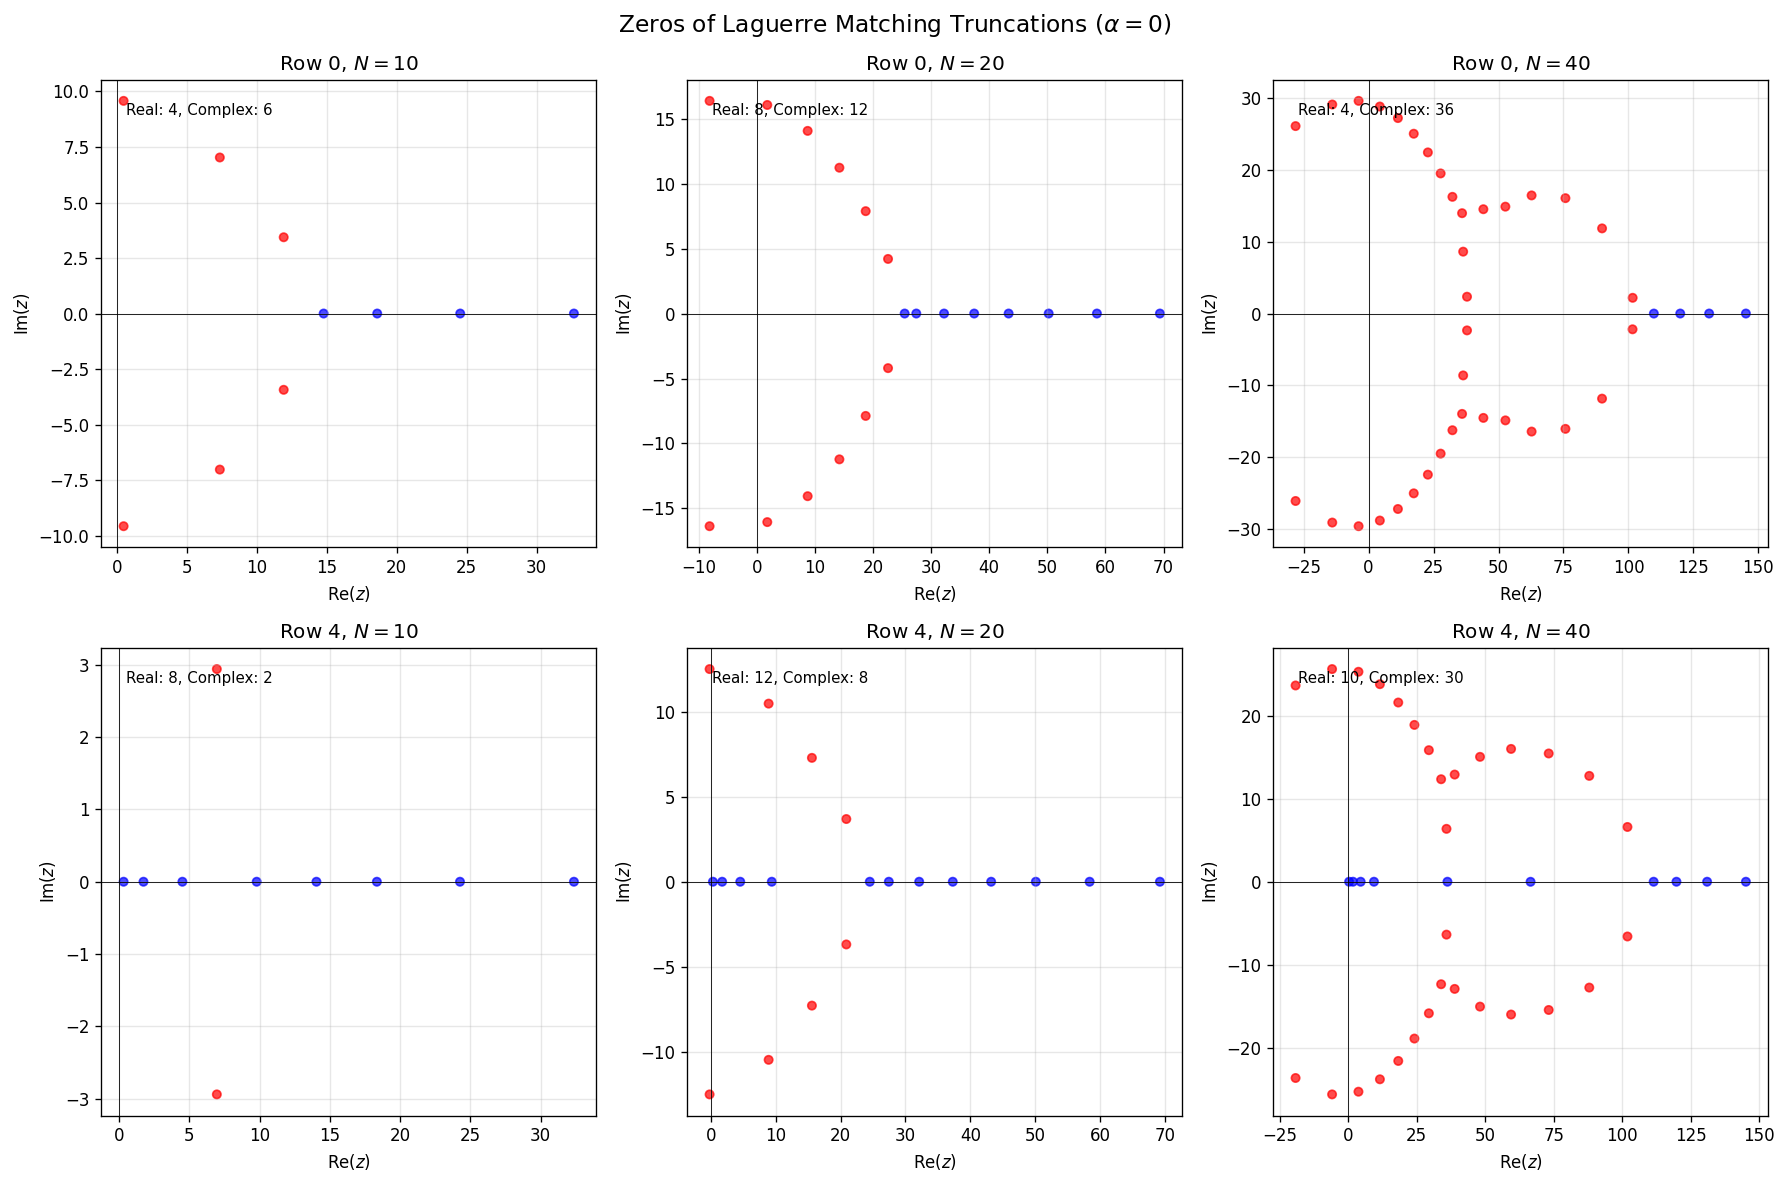
\includegraphics[width=\textwidth]{laguerre_zeros.png}
\caption{Zeros of $f_{r,N}(x) = \sum_{k=0}^N b_{rk}^0\hat{L}_k^{(0)}(x)$
for $r\in\{0,4\}$ and $N\in\{10,20,40\}$.
Blue circles: real positive zeros. Red circles: complex zeros.
All zeros lie in the right half-plane.}
\label{fig:zeros}
\end{figure}

%% ===================================================================
\section{Discussion}
%% ===================================================================

The Laguerre matching matrix for $\alpha=0$ is qualitatively simpler
than its Hermite and Meixner--Pollaczek counterparts:

\begin{center}
\small
\begin{tabular}{lccc}
\toprule
Property & Hermite & Laguerre $\alpha=0$ & MP $\lambda=1/4$ \\
\midrule
GF type & Exponential-quadratic & Rational & $K_0$-Bessel \\
Decay (first row) & Geometric ($3^{-k/2}$) & Geometric ($3^{-(k+1)}$) & Power law \\
Integer rescaling & $D_{mk}/3^{(m+k)/2}$ & $E_{mk} = 3^{m+k+1}b_{mk}/2$ & $T_{mk}\in\Z A\oplus\Z B$ \\
Diagonal GF & $1/\sqrt{(1-3x)(1+x)}$ & $1/\sqrt{(1-t)(1-9t)}$ & None known \\
\bottomrule
\end{tabular}
\end{center}

\noindent The exact decay ratio $1/3$ per index (first-row entries $b_{0k}^0 = 2/3^{k+1}$)
is simpler than Hermite's $3^{-k/2}$ and reflects the fact that the
Laguerre GF poles are at $w=1$ and $u=3$ (from $3-w-u-wu=0$), while
the Hermite GF decays by $e^{-u^2/3}$.

For $\alpha\ne 0$, the rational GF of $\alpha=0$ acquires a fractional
power $(3-w-u-wu)^{3\alpha/2+1}$; the generating function remains
\emph{algebraic} in $(w,u)$ for all rational $\alpha$, but the natural
integrality (which exists for $\alpha=0$ via the integer matrix $E_{mk}$)
breaks. For $\alpha=-\tfrac12$, the entries of $b_{mk}/b_{00}$ appear
to lie in $\Q(\sqrt{2})$, suggesting a two-generator structure over
this quadratic field. For $\alpha=+\tfrac12$, sign oscillations prevent
a clean positive-definite structure.

The combinatorial interpretation of $E_{mk}$ as $q=3$ Delannoy
path counts (Theorem~\ref{thm:inject}) gives a purely bijective proof
of integrality and positivity. It would be interesting to give a
direct bijective proof of the identity
$E_{nn} = \sum_k\binom{n}{k}^2 4^k$ via a bijection between
$q=3$ Delannoy paths of shape $(n,n)$ and pairs of subsets weighted by~$4^k$.

%% ===================================================================
\appendix
\section{Exact Tables}
%% ===================================================================

\begin{table}[ht]
\centering
\caption{The rational table $b_{mk}^0$ (first 6 rows and columns).
All entries are of the form $2r/3^{m+k+1}$ for $r\in\Z_{>0}$.}
\label{tab:bmk}
\small
\begin{tabular}{r|rrrrrr}
\toprule
$m\backslash k$ & $0$ & $1$ & $2$ & $3$ & $4$ & $5$ \\
\midrule
$0$ & $2/3$ & $2/9$ & $2/27$ & $2/81$ & $2/243$ & $2/729$ \\
$1$ & $2/9$ & $10/27$ & $2/9$ & $26/243$ & $34/729$ & $14/729$ \\
$2$ & $2/27$ & $2/9$ & $22/81$ & $146/729$ & $86/729$ & $134/2187$ \\
$3$ & $2/81$ & $26/243$ & $146/729$ & $490/2187$ & $1186/6561$ & $2362/19683$ \\
$4$ & $2/243$ & $34/729$ & $86/729$ & $1186/6561$ & $3842/19683$ & $3254/19683$ \\
$5$ & $2/729$ & $14/729$ & $134/2187$ & $2362/19683$ & $3254/19683$ & $1150/6561$ \\
\bottomrule
\end{tabular}
\end{table}

\begin{table}[ht]
\centering
\caption{The integer matrix $E_{mk}$ (first 8 rows and columns).}
\label{tab:Emk}
\small
\begin{tabular}{r|rrrrrrrr}
\toprule
$m\backslash k$ & $0$ & $1$ & $2$ & $3$ & $4$ & $5$ & $6$ & $7$ \\
\midrule
$0$ & $1$ & $1$ & $1$ & $1$ & $1$ & $1$ & $1$ & $1$ \\
$1$ & $1$ & $5$ & $9$ & $13$ & $17$ & $21$ & $25$ & $29$ \\
$2$ & $1$ & $9$ & $33$ & $73$ & $129$ & $201$ & $289$ & $393$ \\
$3$ & $1$ & $13$ & $73$ & $245$ & $593$ & $1181$ & $2073$ & $3333$ \\
$4$ & $1$ & $17$ & $129$ & $593$ & $1921$ & $4881$ & $10497$ & $20049$ \\
$5$ & $1$ & $21$ & $201$ & $1181$ & $4881$ & $15525$ & $40665$ & $92205$ \\
$6$ & $1$ & $25$ & $289$ & $2073$ & $10497$ & $40665$ & $127905$ & $342105$ \\
$7$ & $1$ & $29$ & $393$ & $3333$ & $20049$ & $92205$ & $342105$ & $1067925$ \\
\bottomrule
\end{tabular}
\end{table}

\begin{table}[ht]
\centering
\caption{Diagonal $E_{nn}$, $n=0,\ldots,15$.
OGF: $1/\sqrt{(1-t)(1-9t)}$.}
\label{tab:diag}
\small
\begin{tabular}{r|r||r|r}
\toprule
$n$ & $E_{nn}$ & $n$ & $E_{nn}$ \\
\midrule
$0$ & $1$ & $8$ & $9\,004\,545$ \\
$1$ & $5$ & $9$ & $76\,499\,525$ \\
$2$ & $33$ & $10$ & $653\,808\,673$ \\
$3$ & $245$ & $11$ & $5\,614\,995\,765$ \\
$4$ & $1\,921$ & $12$ & $48\,416\,454\,529$ \\
$5$ & $15\,525$ & $13$ & $418\,895\,174\,885$ \\
$6$ & $127\,905$ & $14$ & $3\,634\,723\,102\,113$ \\
$7$ & $1\,067\,925$ & $15$ & $31\,616\,937\,184\,725$ \\
\bottomrule
\end{tabular}
\end{table}

\begin{table}[ht]
\centering
\caption{Numerical values $b_{mk}^{-1/2}$ (alpha=$-1/2$, first $5\times 5$)
and $b_{mk}^{+1/2}$ (alpha=$+1/2$, first $5\times 5$), computed to 8 digits.
Note: $b_{00}^{-1/2} = \Gamma(1/4)/(3/2)^{1/4}/\sqrt{\pi} \approx 1.8483462$;
$b_{00}^{+1/2} = \Gamma(7/4)/(3/2)^{7/4}/\Gamma(3/2) \approx 0.5100825$.
Ratio table $F_{mk}^{-1/2}=b_{mk}^{-1/2}/b_{00}^{-1/2}$ has selected
exact values $F_{01}=\sqrt{2}/3$, $F_{11}=4/9$, $F_{22}=17/54$.}
\label{tab:alpha-half}
\small
\begin{tabular}{r|rrrrr}
\toprule
\multicolumn{6}{c}{$\alpha=-1/2$} \\
$m\backslash k$ & $0$ & $1$ & $2$ & $3$ & $4$ \\
\midrule
$0$ & $1.848346$ & $0.871319$ & $0.586899$ & $0.459225$ & $0.388655$ \\
$1$ & $0.871319$ & $0.821487$ & $0.592857$ & $0.432962$ & $0.337499$ \\
$2$ & $0.586899$ & $0.592857$ & $0.581887$ & $0.479110$ & $0.375792$ \\
$3$ & $0.459225$ & $0.432962$ & $0.479110$ & $0.471595$ & $0.410982$ \\
$4$ & $0.388655$ & $0.337499$ & $0.375792$ & $0.410982$ & $0.405778$ \\
\midrule
\multicolumn{6}{c}{$\alpha=+1/2$} \\
$m\backslash k$ & $0$ & $1$ & $2$ & $3$ & $4$ \\
\midrule
$0$ & $0.510082$ & $0.138827$ & $0.010348$ & $-0.022353$ & $-0.025465$ \\
$1$ & $0.138827$ & $0.302271$ & $0.160526$ & $0.048670$ & $-0.003107$ \\
$2$ & $0.010348$ & $0.160526$ & $0.223555$ & $0.151909$ & $0.067602$ \\
$3$ & $-0.022353$ & $0.048670$ & $0.151909$ & $0.184721$ & $0.140266$ \\
$4$ & $-0.025465$ & $-0.003107$ & $0.067602$ & $0.140266$ & $0.161038$ \\
\bottomrule
\end{tabular}
\end{table}

\end{document}
